%\documentclass[12pt,a4paper]{article}
%\usepackage[latin1]{inputenc}
%\usepackage{amsmath}
%\usepackage{amsfonts}
%\usepackage{amssymb}
%\usepackage{graphicx}
%\author{Iason Filippopoulos \and Francky Catthoor \and Per Gunnar Kjeldsberg}
%\title{Technology scaling impact on the interconnect of clustered scratchpad memory architectures}

%\begin{document}
%\maketitle


\chapter{Technology scaling impact on the interconnection of clustered scratchpad memory architectures}

\begin{center}
Iason Filippopoulos, Francky Catthoor, Per Gunnar Kjeldsberg
\\
To be submitted
\\
2015
\end{center}
\afterpage{\null\newpage}
\newpage

\vspace*{\fill}
\section*{\hspace*{\fill} Abstract \hspace*{\fill}}
This work
\vspace*{\fill}
\afterpage{\null\newpage}
\newpage

\section{Introduction}

Power will be the key limiter to  as interconnection networks take up an increasingly significant portion of system power. 

\section{Related Work}

\section{Current technology}
\label{Current}

\subsection{Generic Work-flow}

The current technology is studied as a first step towards the development of an interconnection cost model. 
CAD tools allow the design of the described clustered memory architectures.
The synthesis and the simulation provide reliable data for the area and the power consumption of the different parts of the memory architecture.
The goal is to synthesize a clustered memory architecture and extract power data for the memory banks and the interconnection logic separately.
The work-flow is divided in several sub-steps:

\begin{itemize}
	\item A number of memory banks is chosen from a library, which contains several SotA designs.
	\item An RTL description for connecting the memory banks into a full memory architecture design is written.
	\item A simulation is performed to verify the correct functionality of the memory architecture.
	\item A target technology is chosen and the logic synthesis of the memory architecture is performed.
	\item The floor-planning and the placing \& routing of the memory design is performed.
	\item The dynamic timing and the power simulation are performed and the results are provided.
\end{itemize}

Regarding the first step, the memory models include existing state-of-the-art memories, available from industry and academia, presented in \cite{filippopoulos2013exploration}.
For the memory banks based on the commercial SRAM memories, the energy numbers are derived from a commercial memory compiler.
For the memory banks based on the experimental standard cell-based memories (SCMEM) \cite{Mei11},  the energy numbers are result of synthesis.

For the second step, the RTL description connects the memories using MUX, signals and other components into a functional clustered memory architecture. 
On the third step, the simulation and the verification performs a flash-write followed by a read on the whole memory architecture. 
The target technology depends on the available libraries.
In this work, the TSMC library on 45nm is used.
The place and route can be either performed automatically through the CAD tool or manually by the designer.

The final step, includes the extraction of  parasitic, the static timing analysis and the annotation of the timing to the netlist.
Afterwords, power simulations on the synthesized design are carried out using Synopsys PrimeTime, in order to obtain energy numbers.

\subsection{Example design: synthesis and simulation}

A group of clustered memory architectures is designed and synthesized following the presented work-flow.
The simulation provides results for the current technology and the contribution of the interconnection to the overall energy consumption.
The study includes clustered memories with an increasing number of memory banks, beginning with only one memory bank and continue up to five memory banks.
The breakdown of energy consumption is split into two parts of the memory.
The first part is the energy consumption inside each memory bank, which includes the memory cells, the necessary logic to connect the cells and the addressing circuit.
The second part is the interconnection cost between the different memory banks, which includes the necessary logic to locate and transfer the data outside of the banks. 
In other words, the interconnection outside the memory banks is given separately. 
The interconnection between the different memory cells inside one bank is included on the energy of the memory bank.

The energy breakdown between the first part of the memory banks and the second part of the interconnection (part2) is presented in Fig.\ref{fig:energyE}.
The energy cost of the interconnection logic is small compared to the energy cost for the write and read operations on the memory banks.
Tab.\ref{tab:overhead} contains the exact percentages of the energy overhead on the interconnection. 

\begin{figure}
 \centering
 \includegraphics[width = \textwidth]{E/energy.pdf}
  \caption{Energy breakdown between the memory banks and the interconnection}
 \label{fig:energyE}
 \end{figure}
 
 \begin{figure}
 \centering
 \includegraphics[width = \textwidth]{E/area.pdf}
  \caption{Area breakdown between the memory banks and the interconnection}
 \label{fig:areaE}
 \end{figure}
 
 \begin{table}[t!]
\caption{Percentage of energy overhead on interconnection}
\label{tab:overhead}
\centering
\begin{tabular}{|c|c|c|c|c|c|}
\hline 
Banks & 1 & 2 & 3 & 4 & 5 \\
\hline 
Overhead(\%) & 0	&	1.2627 & 1.3687 & 1.7683 & 3.0067 \\ 
 \hline 
 \end{tabular} 
\end{table} 
 
The changes in the area of the design is presented in Fig.\ref{fig:areaE}.
The area used for the placement of the memory banks is separated from the area occupied by the interconnection.
  
In addition, the synthesis and simulation of the memory designs provide useful information about the dimensions of the memory banks, the length and the capacitance of the wires.
Several interesting observations are possible based on the study of the current technology.
The energy overhead on the interconnection of the banks grows when there are more memory banks connected, as expected.
However, the overhead is just over 3\% even for a clustered memory with five banks. 
The area overhead is significantly higher and grows exponentially for an increasing number of memory banks.  
The maximum area overhead is less than 10\%.
This is explained by the need for extra wiring to connect the different memory banks.

\section{Technology Scaling}

The technology scaling projections are based on the reports released by the International Technology Roadmap for Semiconductors (ITRS) \cite{itrs}.
The clustered memory architecture can be divided into two parts, i.e. the memory banks and the interconnection.

\subsection{Memory Banks}

The memory banks consist of the memory cells, which are built using gates.
Thus, the predictions about the future behavior of the memory banks is based on the ITRS reports for logic.
In the following years, the gate of the length is expected to be reduced as shown in \ref{fig:gateE}.
The values are approaching 5nm around 2028, which is potentially the limit using the current manufacturing process.

\begin{figure}
 \centering
 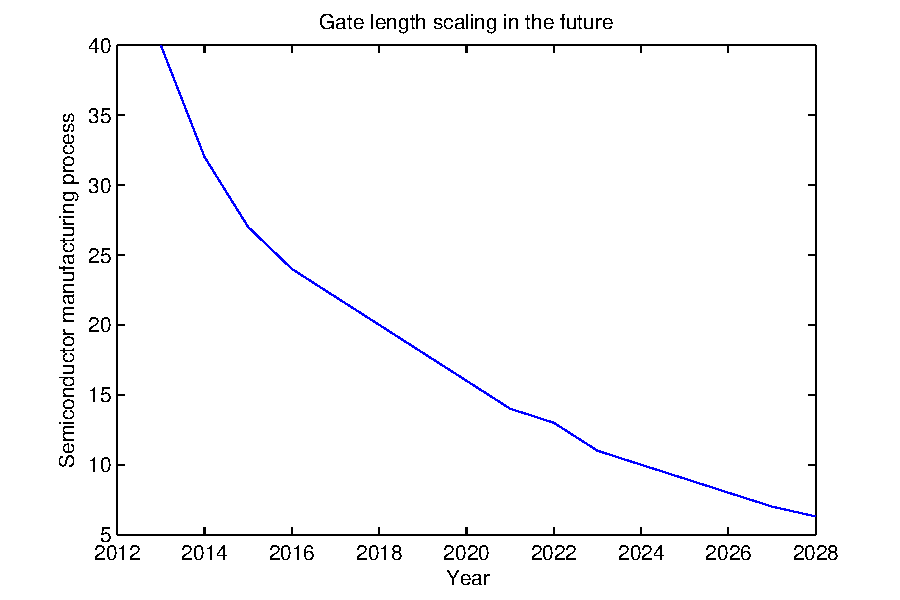
\includegraphics[width = \textwidth]{E/gate.pdf}
  \caption{Impact of technology scaling into gate length}
 \label{fig:gateE}
 \end{figure}
 
 \begin{figure}
 \centering
 \includegraphics[width = \textwidth]{E/cellpower.pdf}
  \caption{Normalized dynamic power and technology scaling}
 \label{fig:powerE}
 \end{figure}

The reduction on the gate length leads to a reduction of the memory cell and naturally smaller memory banks.
The smaller memory banks affect the area of the design and the power consumption.
The projections provided by ITRS regarding the power are presented in \ref{fig:powerE}. 
There is a significant reduction on the power consumption in the short term and slighter reduction at the end of the projections.

\subsection{Interconnection}

The interconnection cost is based on the projections about wiring, which differentiate compared to the projections regarding the logic gates.
However, the change on the size of the memory banks affects the length of the needed wires.
The most important parameters for the current study is the capacitance and the power of the interconnection.
Based on the data provided by ITRS, the curves for the two parameters are presented in \ref{fig:intpowerE}.
The capacitance is expected to be reduced in the following year.
However, the rate of reduction is lower compared to the expected reduction for the memory banks.
The power values are per length unit and there are expected to raise due to the several challenges that the interconnection technology will face in the future.

 \begin{figure}
 \centering
 \includegraphics[width = \textwidth]{E/intpower.pdf}
  \caption{Impact of technology scaling into the capacitance and the power of the interconnection part}
 \label{fig:intpowerE}
 \end{figure}


\section{Model Construction and Projection Results}

 The scope is to develop a model that can provide a rough estimation on the power overhead for the interconnection on clustered memory architectures.
 The model is based on the synthesis results of the currently feasible designs and study of the projections provided by ITRS.
 The input for the model is the process technology and the number of memory banks.
 The power consumption on the memory banks is calculated using Fig.\ref{fig:powerE}.
  The prediction of the power consumption on the interconnection logic is more complex.
 Based on the technology and the number of memory banks, the length of the wires is calculated and sequentially the capacitance.
 Normally the power consumption is given as  $Power = \dfrac{1}{2} \times f \times C \times V^{2} $, where  f is the operating frequency, C the capacitance and V the supply voltage.
 However, the simulation results and the projections provided by ITRS suggest that a more complex model of computation is needed.
 
 The model of computation for the interconnection power cost overhead for a given target technology $ t $ and a number of $ n $ banks of 1KB  is:
 
 \begin{center}
 $ \dfrac{Interconnection_{power}}{MemoryCells_{power}}(t) = \dfrac{C(t,area(n)) \times V^{2} \times W(t) }{n \times Bank_{power}(t)} $ 
  \end{center}
  
 where:

 \begin{itemize}
 \item $C(t,n)$ is the capacitance of the interconnection wires for the given technology and the length of wiring based on the area, which is calculated for the different number of banks
 \item $ W(n) $ is a wiring efficiency factor based on the power curve in \ref{fig:intpowerE}
 \item $ Bank_{power} $ is the power consumption on a memory bank of 1KB for the given technology
 \end{itemize}
 
 The development of the interconnection cost overhead using the proposed model is presented in Fig.\ref{fig:overheadE}.
 The model reproduces the results for the synthesized results presented in \ref{tab:overhead}.

 \begin{figure}
 \centering
 \includegraphics[width = \textwidth]{E/overhead.pdf}
  \caption{Projections of the interconnection cost power overhead for different numbers of memory banks}
 \label{fig:overheadE}
 \end{figure}

\section{Conclusion}

The model reproduces the results for the designs that can be synthesized nowadays and are presented in \ref{Current}. 

The estimations for the future can be useful for system desi

\bibliographystyle{plain}
\bibliography{reference}

%\end{document}
